% =====================================================================
%  An Illustrated Guide to the YOLOv8 Polygon + Distance (TensorFlow) codebase
%  Build:  tectonic main.tex   (or: bash build.sh)
%  Editable source — edit chapters/*.tex and re-run the build.
% =====================================================================
\documentclass[11pt]{report}

\usepackage[a4paper,margin=2.3cm,headsep=10pt]{geometry}
\usepackage{graphicx}
\usepackage{xcolor}
\usepackage{amsmath,amssymb}
\usepackage{booktabs}
\usepackage{array}
\usepackage{enumitem}
\usepackage{microtype}
\usepackage{caption}
\usepackage[most]{tcolorbox}
\usepackage{tikz}
\usetikzlibrary{positioning,arrows.meta,shapes.geometric,fit,backgrounds,calc}
\usepackage{listings}
\usepackage{fancyhdr}
\usepackage[colorlinks=true,linkcolor=accent,urlcolor=accent,citecolor=accent]{hyperref}

% ---------- palette ----------
\definecolor{accent}{HTML}{2563EB}
\definecolor{ink}{HTML}{1E293B}
\definecolor{teal}{HTML}{0891B2}
\definecolor{green}{HTML}{16A34A}
\definecolor{amber}{HTML}{B45309}
\definecolor{amberbg}{HTML}{FEF3C7}
\definecolor{greenbg}{HTML}{DCFCE7}
\definecolor{bluebg}{HTML}{DBEAFE}
\definecolor{redbg}{HTML}{FEE2E2}
\definecolor{red}{HTML}{DC2626}
\definecolor{graybg}{HTML}{F1F5F9}
\definecolor{codebg}{HTML}{F8FAFC}
\definecolor{codekw}{HTML}{7C3AED}
\definecolor{codestr}{HTML}{16A34A}
\definecolor{codecom}{HTML}{64748B}

\color{ink}

% ---------- headers / footers ----------
\pagestyle{fancy}
\fancyhf{}
\renewcommand{\headrulewidth}{0.3pt}
\fancyhead[L]{\small\textcolor{accent}{\leftmark}}
\fancyhead[R]{\small YOLOv8 Poly + Distance}
\fancyfoot[C]{\small\thepage}

% ---------- listings ----------
\lstdefinestyle{base}{
  backgroundcolor=\color{codebg},
  basicstyle=\ttfamily\small\color{ink},
  keywordstyle=\color{codekw}\bfseries,
  stringstyle=\color{codestr},
  commentstyle=\color{codecom}\itshape,
  numberstyle=\tiny\color{codecom},
  frame=single, rulecolor=\color{black!15},
  breaklines=true, showstringspaces=false,
  columns=fullflexible, keepspaces=true,
  xleftmargin=10pt, xrightmargin=6pt, framexleftmargin=8pt,
  aboveskip=8pt, belowskip=6pt,
}
\lstdefinestyle{py}{style=base,language=Python,morekeywords={tf,self,None,True,False}}
\lstdefinestyle{bash}{style=base,language=bash}
\lstset{style=base}
% YAML-ish
\lstdefinelanguage{yaml}{keywords={true,false,null},comment=[l]{\#},morestring=[b]'}

% ---------- callout boxes ----------
\newtcolorbox{teacher}[1][]{enhanced,breakable,colback=greenbg,colframe=green,
  coltitle=white,boxrule=0.4pt,arc=2pt,left=8pt,right=8pt,top=5pt,bottom=5pt,
  fonttitle=\bfseries,title={\faGraduationCap\ Beginner's note},#1}
\newtcolorbox{hood}[1][]{enhanced,breakable,colback=bluebg,colframe=accent,
  coltitle=white,boxrule=0.4pt,arc=2pt,left=8pt,right=8pt,top=5pt,bottom=5pt,
  fonttitle=\bfseries,title={Under the hood},#1}
\newtcolorbox{why}[1][]{enhanced,breakable,colback=amberbg,colframe=amber,
  coltitle=white,boxrule=0.4pt,arc=2pt,left=8pt,right=8pt,top=5pt,bottom=5pt,
  fonttitle=\bfseries,title={Why this codebase does it this way},#1}
\newtcolorbox{pitfall}[1][]{enhanced,breakable,colback=redbg,colframe=red,
  coltitle=white,boxrule=0.4pt,arc=2pt,left=8pt,right=8pt,top=5pt,bottom=5pt,
  fonttitle=\bfseries,title={Gotcha},#1}
% graduation-cap glyph fallback (no fontawesome dependency)
\newcommand{\faGraduationCap}{\textbf{\textsf{>}}}

% ---------- tikz styles ----------
\tikzset{
  blk/.style={rectangle,rounded corners=3pt,draw=accent,fill=bluebg,
    align=center,inner sep=5pt,font=\small,minimum height=8mm},
  blkg/.style={rectangle,rounded corners=3pt,draw=green,fill=greenbg,
    align=center,inner sep=5pt,font=\small,minimum height=8mm},
  blka/.style={rectangle,rounded corners=3pt,draw=amber,fill=amberbg,
    align=center,inner sep=5pt,font=\small,minimum height=8mm},
  blkn/.style={rectangle,rounded corners=3pt,draw=black!40,fill=graybg,
    align=center,inner sep=5pt,font=\small,minimum height=8mm},
  ar/.style={-{Stealth[length=2.2mm]},thick,draw=ink},
  lbl/.style={font=\scriptsize\itshape,text=codecom},
}

\newcommand{\code}[1]{\texttt{\small #1}}
\newcommand{\file}[1]{\textcolor{teal}{\texttt{\small #1}}}

% ---------- figure helper ----------
\newcommand{\guidefig}[3]{% file, width-frac, caption
  \begin{figure}[ht]\centering
    \includegraphics[width=#2\linewidth]{figures/#1}
    \caption{#3}\end{figure}}

\captionsetup{font=small,labelfont={bf,color=accent}}

% =====================================================================
\begin{document}

% ---------------- Title page ----------------
\begin{titlepage}
\centering
\vspace*{1.2cm}
{\Huge\bfseries\color{accent} An Illustrated Guide\par}
\vspace{4mm}
{\LARGE to the YOLOv8 Polygon + Distance codebase\par}
\vspace{2mm}
{\large\itshape A TensorFlow reimplementation — explained from scratch\par}
\vspace{10mm}

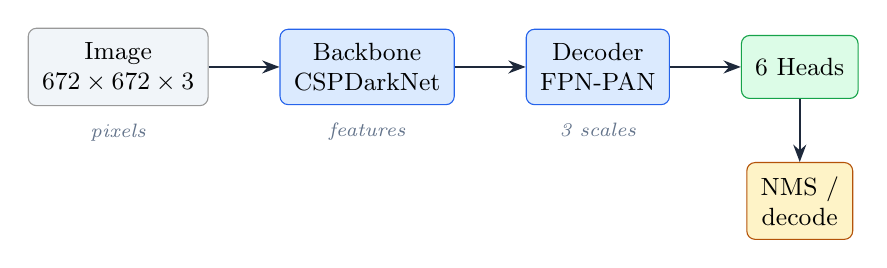
\begin{tikzpicture}[node distance=6mm and 9mm]
  \node[blkn] (img) {Image\\$672\times672\times3$};
  \node[blk,right=of img] (bb) {Backbone\\CSPDarkNet};
  \node[blk,right=of bb] (dec) {Decoder\\FPN-PAN};
  \node[blkg,right=of dec] (head) {6 Heads};
  \node[blka,below=8mm of head] (nms) {NMS /\\decode};
  \draw[ar] (img)--(bb); \draw[ar] (bb)--(dec); \draw[ar] (dec)--(head);
  \draw[ar] (head)--(nms);
  \node[lbl,below=1mm of img] {pixels};
  \node[lbl,below=1mm of bb] {features};
  \node[lbl,below=1mm of dec] {3 scales};
\end{tikzpicture}

\vspace{12mm}
{\large Detection \quad$\bullet$\quad Polygon segmentation \quad$\bullet$\quad Distance estimation\par}
\vspace{4mm}
{\color{codecom}\small 39 classes \;|\; 6 output heads \;|\; PolyYOLO 24-vertex radial polygons \;|\; per-object distance}
\vfill
{\small This guide is generated from the project's own code and docs. Every
``real-pipeline'' figure is produced by running the actual augmentation / model
code (see \file{docs/codebase\_guide/gen\_figures.py}). Edit \file{chapters/*.tex} and
rebuild to change it.\par}
\vspace{6mm}
\end{titlepage}

% ---------------- TOC ----------------
\tableofcontents
\thispagestyle{fancy}

\chapter*{How to read this guide}
\addcontentsline{toc}{chapter}{How to read this guide}
\markboth{How to read this guide}{}

Welcome! This guide explains an entire deep-learning codebase --- a TensorFlow
reimplementation of \textbf{YOLOv8} that also predicts \textbf{object outlines}
(polygons) and \textbf{how far away} each object is. It is written for someone who
is comfortable with Python but is \emph{new} to object detection. We start from the
ideas, then walk through the actual code, file by file.

\section*{Who this is for}
You will get the most out of this if you know basic Python and a little about neural
networks (``a model takes an input, has weights, and is trained with gradient
descent''). You do \emph{not} need prior knowledge of object detection, anchors,
IoU, segmentation, or YOLO. Every such term is introduced when first used.

\section*{The four kinds of callout boxes}
Throughout the guide you will see colored boxes. Each has a job:

\begin{teacher}
Explains a concept from scratch --- what it means and why it exists. Read these if a
term is new to you.
\end{teacher}

\begin{hood}
Shows the concrete mechanism in \emph{this} codebase: the function, the tensor shape,
the exact formula. Read these to connect the idea to the code.
\end{hood}

\begin{why}
A non-obvious design decision and the reasoning behind it. Several choices here differ
from ``stock'' YOLOv8 on purpose; these boxes say why.
\end{why}

\begin{pitfall}
A subtle trap --- a coordinate-order mismatch, a sentinel value, a normalization
convention --- that causes real bugs if you get it wrong.
\end{pitfall}

\section*{Conventions}
File and symbol names look like \file{data\_pipeline/mosaic.py} and \code{Mosaic.\_mosaic}.
Tensor shapes are written \code{[N, 72]}. Where coordinates matter we always say which
convention is in play --- \code{yxyx} vs \code{xyxy}, normalized \code{[0,1]} vs pixels ---
because mixing them up is the single most common source of bugs in this kind of code.

\section*{A map of the journey}
\begin{enumerate}[leftmargin=1.4em,itemsep=2pt]
  \item \textbf{Foundations} --- the object-detection ideas you need (boxes, IoU, NMS,
        anchors, feature pyramids, segmentation, the YOLO idea).
  \item \textbf{The system at a glance} --- the three model tiers and the six heads.
  \item \textbf{The data pipeline} --- how images and labels are loaded and augmented.
  \item \textbf{Polygons} --- the radial ``PolyYOLO'' representation, in depth.
  \item \textbf{The model} --- backbone, decoder, heads, and post-processing.
  \item \textbf{The losses} --- task-aligned assignment and every loss term.
  \item \textbf{Training} --- optimizer, schedules, EMA, the training loop.
  \item \textbf{Configuration, evaluation, tooling} --- how to actually run it.
\end{enumerate}

\noindent Let's begin.

\chapter{Foundations: the ideas behind object detection}

This chapter builds the vocabulary. If you already know what IoU, anchors, NMS, feature
pyramids, and segmentation are, you can skim. Otherwise, read it once and the code
chapters will read much more easily.

\section{What ``object detection'' actually asks for}
Image \emph{classification} answers ``what is in this picture?'' with a single label.
\textbf{Object detection} is harder: it must answer ``\emph{what} objects are here, and
\emph{where} is each one?'' --- producing, for every object, a \textbf{bounding box}
(a rectangle) and a \textbf{class label}. This codebase then adds two more questions per
object: ``what is its exact outline?'' and ``how far away is it?''.

\section{Bounding boxes and coordinate conventions}
A box is four numbers. But there are several ways to write those four numbers, and mixing
them up is the \#1 bug in detection code.

\begin{center}
\renewcommand{\arraystretch}{1.25}
\begin{tabular}{l l}
\toprule
\textbf{Convention} & \textbf{The four numbers} \\
\midrule
\code{xyxy} & left, top, right, bottom (two corners), x first \\
\code{yxyx} & top, left, bottom, right (two corners), y first \\
\code{xywh} & center-x, center-y, width, height \\
normalized & each value divided by image width/height, so in $[0,1]$ \\
pixels      & raw pixel coordinates \\
\bottomrule
\end{tabular}
\end{center}

\begin{pitfall}
This repo deliberately uses \textbf{two} conventions and converts between them at a known
seam. Ground-truth boxes coming out of the dataset decoders and parsers are
\code{yxyx}, \textbf{normalized} to $[0,1]$. The loss and the label-assignment code
convert to \code{xyxy} in \textbf{pixels}. Whenever you touch box math, first ask
``which convention am I in?''. The codebase is careful to label this everywhere; you
should be too.
\end{pitfall}

\section{Intersection over Union (IoU)}
To say whether a predicted box is ``correct'', we need to measure how well it overlaps a
ground-truth box. The standard measure is \textbf{Intersection over Union}: the area of
overlap divided by the area of their union.

\begin{center}
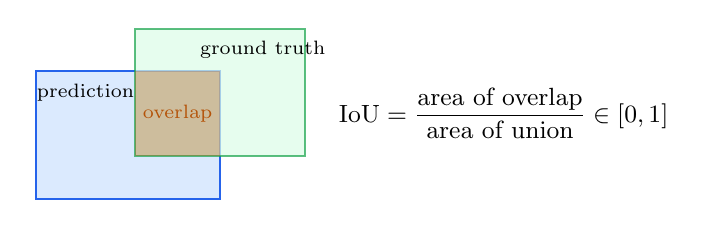
\begin{tikzpicture}[scale=0.9]
  \fill[bluebg,draw=accent,thick] (0,0) rectangle (2.6,1.8);
  \fill[greenbg,draw=green,thick,opacity=0.7] (1.4,0.6) rectangle (3.8,2.4);
  \fill[amber,opacity=0.35] (1.4,0.6) rectangle (2.6,1.8);
  \node[font=\scriptsize] at (0.7,1.5) {prediction};
  \node[font=\scriptsize] at (3.2,2.1) {ground truth};
  \node[font=\scriptsize,text=amber] at (2.0,1.2) {overlap};
  \node[font=\small] at (6.6,1.2) {$\text{IoU}=\dfrac{\text{area of overlap}}{\text{area of union}}\in[0,1]$};
\end{tikzpicture}
\end{center}

\noindent IoU is 1 for a perfect match and 0 for no overlap. A common rule is ``a
detection counts as correct if its IoU with a true box is at least 0.5''. IoU appears
everywhere: in the metric that scores the model, in NMS, and --- in a refined form called
\textbf{CIoU} --- inside the box loss.

\section{Confidence scores and NMS}
Each detection comes with a \textbf{confidence} (or score) in $[0,1]$: how sure the model
is. A detector fires on the same object from several adjacent grid cells, so we get a
cluster of overlapping boxes. \textbf{Non-maximum suppression} cleans this up: sort by
score, keep the top box, delete every other box that overlaps it too much (IoU above a
threshold), repeat.

\begin{hood}
Here NMS runs in \file{models/detection\_generator.py} with \code{max\_boxes=300},
\code{nms\_thresh=0.65}, \code{score\_thresh=0.05}, and it is \textbf{per-class}: classes
do not suppress each other, so an overlapping ``person'' and ``bag'' both survive.
\end{hood}

\section{The grid idea: how YOLO predicts}
YOLO (``You Only Look Once'') does not propose-then-classify. It overlays a \textbf{grid}
on the feature map and asks \emph{every cell} to predict whether an object is centered
there, and if so its box, class, and (here) polygon and distance. One forward pass yields
all predictions --- fast and simple.

\begin{teacher}
\textbf{Stride.} A backbone shrinks the image. If a feature map is 8$\times$ smaller than
the input, we say it has \textbf{stride 8}: each cell ``sees'' an $8\times8$ pixel patch.
Small strides (fine grids) catch small objects; large strides (coarse grids) catch large
ones.
\end{teacher}

\section{Feature pyramids and multiple scales}
A single grid can't handle a tiny sign and a huge truck equally well. So detectors use a
\textbf{feature pyramid}: several feature maps at different strides. This codebase uses
three, at strides \textbf{8, 16, and 32} (grids of $84\times84$, $42\times42$,
$21\times21$ for a 672-pixel input). Every head predicts at all three. The decoder that
builds and fuses these maps is an \textbf{FPN-PAN} --- covered in the architecture chapter.

\section{Anchor-free detection}
Older detectors placed several preset box shapes (``anchors'') at each cell and predicted
offsets from them. YOLOv8 is \textbf{anchor-free}: each cell has a single \emph{anchor
point} at its center, and the box head predicts the distances from that point to the four
sides. The anchor points are simply the cell centers, $(i+0.5)\cdot\text{stride}$,
built inside the loss and the detection generator.

\section{Two ways to describe an object's shape}
A bounding box is a crude outline. \textbf{Segmentation} describes the actual shape. There
are two common encodings:

\begin{itemize}[leftmargin=1.4em,itemsep=2pt]
  \item a \textbf{mask} --- a per-pixel ``inside/outside'' map (heavy, but exact);
  \item a \textbf{polygon} --- an ordered list of boundary points (compact).
\end{itemize}

\noindent This codebase uses a special \emph{radial} polygon format from
``PolyYOLO'': 24 vertices arranged at fixed $15^\circ$ angles around the box center. It
is light enough to predict with three small heads and is the subject of
Chapter~\ref{ch:polygons}.

\section{Estimating distance}
The last extra task is \textbf{monocular distance estimation}: from a single RGB image,
predict how far each object is, in meters. This is learned from a separate labeled dataset
and predicted by a one-channel head on a log scale. It is trained jointly with detection,
merged at the batch level --- a neat trick we will see in the data-pipeline chapter.

\section{How a model ``learns where things are''}
One subtlety underlies all of detection training. The model makes predictions at thousands
of grid cells, but a training image has only a handful of objects. Which cells should be
held responsible for which object? This is \textbf{label assignment}, and modern YOLO uses
a smart, learnable scheme called \textbf{Task-Aligned Assignment (TAL)} that picks, for
each object, the cells whose predictions are already both well-localized and
well-classified. We devote a section to it in the losses chapter --- it is the heart of how
the model is trained.

\medskip
\noindent That is the whole vocabulary. Armed with it, let's open the codebase.

\chapter{The system at a glance}

Before diving into any single file, let's see the whole machine. This codebase takes a
$672\times672$ RGB image and, in one forward pass, predicts three things for every
object it finds:

\begin{enumerate}[leftmargin=1.4em,itemsep=1pt]
  \item a \textbf{bounding box} and a \textbf{class} (this is ordinary object detection);
  \item a \textbf{polygon outline} of the object (segmentation);
  \item the \textbf{distance} to the object in meters.
\end{enumerate}

It is a faithful TensorFlow~2.16 re-implementation of Ultralytics YOLOv8, extended with
two extra prediction ``heads''. The assembly happens in \file{models/yolo\_v8.py}
(\code{build\_yolov8}).

\section{The end-to-end path}
Every image flows through four stages:

\begin{center}
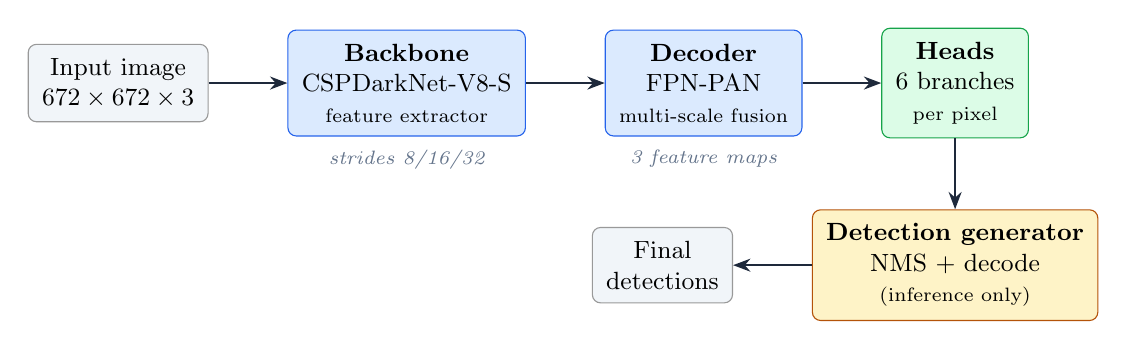
\begin{tikzpicture}[node distance=7mm and 10mm]
  \node[blkn] (img) {Input image\\$672\times672\times3$};
  \node[blk,right=of img] (bb) {\textbf{Backbone}\\CSPDarkNet-V8-S\\\scriptsize feature extractor};
  \node[blk,right=of bb] (dec) {\textbf{Decoder}\\FPN-PAN\\\scriptsize multi-scale fusion};
  \node[blkg,right=of dec] (head) {\textbf{Heads}\\6 branches\\\scriptsize per pixel};
  \node[blka,below=9mm of head] (nms) {\textbf{Detection generator}\\NMS + decode\\\scriptsize (inference only)};
  \node[blkn,left=of nms] (out) {Final\\detections};
  \draw[ar] (img)--(bb); \draw[ar] (bb)--(dec); \draw[ar] (dec)--(head);
  \draw[ar] (head)--(nms); \draw[ar] (nms)--(out);
  \node[lbl,below=0.5mm of bb] {strides 8/16/32};
  \node[lbl,below=0.5mm of dec] {3 feature maps};
\end{tikzpicture}
\end{center}

\begin{teacher}
A \textbf{backbone} is a stack of convolutional layers that turns raw pixels into
compact ``feature maps'' --- grids of numbers where each cell summarizes a patch of the
image. A \textbf{decoder} (here a feature pyramid) mixes information across resolutions
so the model can see both small and large objects. The \textbf{heads} are the final
thin layers that read those features and output the actual predictions. We unpack each
of these in the architecture chapter.
\end{teacher}

\section{Three tiers, one codebase}
The same code supports three configurations, chosen by an experiment YAML file. They
differ only in which heads are turned on:

\begin{center}
\renewcommand{\arraystretch}{1.3}
\begin{tabular}{>{\raggedright\arraybackslash}p{4.5cm} l l}
\toprule
\textbf{Config (\file{configs/experiments/yolo/})} & \textbf{Heads} & \textbf{Task} \\
\midrule
\file{yolov8\_bbox.yaml}      & box + cls & detection only \\
\file{yolov8\_poly.yaml}      & box + cls + polygon & detection + segmentation \\
\file{yolov8\_poly\_dist.yaml} & all 6 heads & detection + segmentation + distance \\
\bottomrule
\end{tabular}
\end{center}

\noindent The full tier, \file{yolov8\_poly\_dist.yaml}, is the authoritative reference
configuration --- when in doubt about a hyperparameter, that file is the source of truth.

\section{The six heads}
Every head produces a prediction at \emph{every pixel} of \emph{every} one of the three
feature-map scales. Here is what each one outputs.

\begin{center}
\renewcommand{\arraystretch}{1.3}
\begin{tabular}{l c >{\raggedright\arraybackslash}p{8.2cm}}
\toprule
\textbf{Head} & \textbf{Channels} & \textbf{Meaning} \\
\midrule
\code{box}        & 64 & box position, as a ``distribution'' --- 4 sides $\times$ 16 bins (DFL) \\
\code{cls}        & 39 & one logit per class \\
\code{poly\_angle} & 24 & per-vertex sub-bin angle offset (one per polygon bin) \\
\code{poly\_dist}  & 24 & per-vertex radial distance (one per polygon bin) \\
\code{poly\_conf}  & 24 & per-vertex ``is there a vertex here?'' gate \\
\code{dist}       & 1  & object distance, on a log scale \\
\bottomrule
\end{tabular}
\end{center}

\begin{hood}
The heads live in \file{models/head.py} (\code{YoloV8Head}). The three polygon heads
(\code{poly\_angle}, \code{poly\_dist}, \code{poly\_conf}) together encode a 24-vertex
outline in the ``radial'' PolyYOLO format --- the subject of its own chapter. The
\code{box} head's 64 channels are $4\times16$: each of the four box sides is predicted
as a little probability distribution over 16 distance bins, a trick called
\emph{Distribution Focal Loss}. The heads are pinned to \code{float32} even when the
rest of the model runs in \code{mixed\_bfloat16}.
\end{hood}

\section{What ``training'' produces}
During training the model runs in a mode where the heads emit \emph{raw} numbers and a
loss compares them to ground-truth labels. During inference (\code{deploy=True}) a final
stage --- the \textbf{detection generator} (\file{models/detection\_generator.py}) ---
decodes those raw numbers into clean boxes, runs \textbf{non-maximum suppression} to
remove duplicates, and converts the polygon and distance outputs into human-readable
form.

\begin{teacher}
\textbf{Non-maximum suppression (NMS)} is a clean-up step. A detector typically fires on
the same object from several neighboring pixels, producing a cluster of overlapping
boxes. NMS keeps the highest-scoring box in each cluster and suppresses the rest, so each
object is reported once.
\end{teacher}

With the map in hand, the next chapter builds up the detection ideas themselves --- so
that when we open the code, every term already means something.

\chapter{The data pipeline}
\label{ch:pipeline}

A model is only as good as the data it sees. This codebase has an unusually rich input
pipeline: it samples from several datasets, augments aggressively, and even merges a
\emph{second} dataset (for distance) into each training batch. Everything lives under
\file{data\_pipeline/} and is assembled in \file{input\_reader.py}.

\begin{teacher}
In TensorFlow, data loading is built as a \code{tf.data} \emph{pipeline}: a chain of
operations (read $\rightarrow$ decode $\rightarrow$ shuffle $\rightarrow$ augment
$\rightarrow$ batch) that streams examples to the GPU. Each stage runs in parallel on CPU
worker threads while the GPU trains on the previous batch, so data prep and training
overlap.
\end{teacher}

\section{The stage order}
Here is the whole detection pipeline, top to bottom. The order is not arbitrary --- each
stage depends on the previous one.

\begin{center}
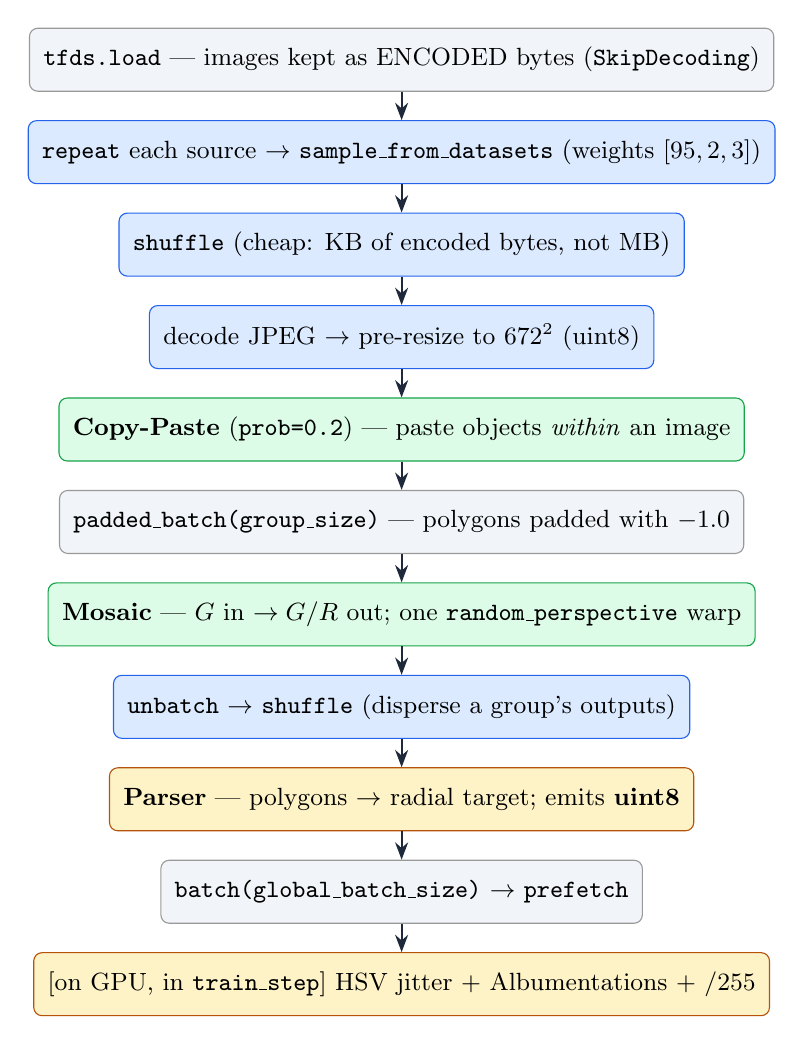
\begin{tikzpicture}[node distance=3.6mm,every node/.style={font=\small}]
  \node[blkn] (load) {\code{tfds.load} --- images kept as ENCODED bytes (\code{SkipDecoding})};
  \node[blk,below=of load] (rep) {\code{repeat} each source $\rightarrow$ \code{sample\_from\_datasets} (weights $[95,2,3]$)};
  \node[blk,below=of rep] (shuf) {\code{shuffle} (cheap: KB of encoded bytes, not MB)};
  \node[blk,below=of shuf] (dec) {decode JPEG $\rightarrow$ pre-resize to $672^2$ (uint8)};
  \node[blkg,below=of dec] (cnp) {\textbf{Copy-Paste} (\code{prob=0.2}) --- paste objects \emph{within} an image};
  \node[blkn,below=of cnp] (pb) {\code{padded\_batch(group\_size)} --- polygons padded with $-1.0$};
  \node[blkg,below=of pb] (mos) {\textbf{Mosaic} --- $G$ in $\rightarrow G/R$ out; one \code{random\_perspective} warp};
  \node[blk,below=of mos] (un) {\code{unbatch} $\rightarrow$ \code{shuffle} (disperse a group's outputs)};
  \node[blka,below=of un] (par) {\textbf{Parser} --- polygons $\rightarrow$ radial target; emits \textbf{uint8}};
  \node[blkn,below=of par] (bat) {\code{batch(global\_batch\_size)} $\rightarrow$ \code{prefetch}};
  \node[blka,below=of bat] (gpu) {[on GPU, in \code{train\_step}] HSV jitter + Albumentations + $/255$};
  \foreach \a/\b in {load/rep,rep/shuf,shuf/dec,dec/cnp,cnp/pb,pb/mos,mos/un,un/par,par/bat,bat/gpu}
    \draw[ar] (\a)--(\b);
\end{tikzpicture}
\end{center}

\begin{hood}
Two design choices keep this fast on a CPU-limited host. (1) \textbf{\code{SkipDecoding}}:
images travel through the shuffle buffer as compressed JPEG bytes (kilobytes), and are
only decoded inside the parallel \code{map} --- a 16k-element shuffle buffer stays cheap
instead of holding gigabytes of decoded pixels. (2) \textbf{Color augmentation is moved
to the GPU}: the parsers emit \code{uint8} images and the HSV/Albumentations/$/255$ work
happens once per batch inside \code{train\_step} (\file{data\_pipeline/batch\_color\_aug.py}),
cutting host$\rightarrow$device traffic $4\times$.
\end{hood}

\section{Sampling from several datasets}
The detection stream is not one dataset but several (\code{cleaner\_polygon2026},
\code{field\_misrecog2026}, \code{station\_misrecog}), blended with fixed
\textbf{sampling weights}. Each source is \code{repeat()}-ed first so the blend is a
stationary, infinite stream --- the weights stay constant forever rather than drifting as
a finite source runs out.

\section{Copy-Paste, then Mosaic}
Two augmentations stitch content together, and \emph{order matters}.

\textbf{Copy-Paste} (\file{copy\_paste.py}) pastes a cut-out object (from a separate RGBA
dataset, the alpha channel being the mask) onto the current image. It runs \emph{first},
because it augments \emph{within} a single image. \textbf{Mosaic} then stitches four
whole images together, so it must come after.

\guidefig{fig_perspective.png}{1.0}{The one geometric transform, \code{random\_perspective}
(rotation, scale, shear, translate), rendered by the actual code in
\file{data\_pipeline/augmentations.py}. The box (blue) and polygon (red) ground truth are
transformed by the same matrix and clipped to the image edge. This same warp is applied to
single images and to mosaics.}

\subsection{Mosaic in depth}
Mosaic builds a $2\times$-size canvas, places four images toward a random center, and then
applies \emph{one} \code{random\_perspective} warp that crops it back to $672\times672$.

\guidefig{fig_mosaic.png}{1.0}{The real \code{Mosaic.\_mosaic} output. Four source images
are resized and placed into the four quadrants of a $1344\times1344$ canvas, then a single
warp produces the final image. Ground-truth boxes and polygons are carried through the
\emph{same} matrix, so labels stay perfectly aligned.}

\begin{why}
The mosaic assembles a canvas and warps \emph{once}, rather than warping each of the four
source images separately and compositing. The two are geometrically identical, but the
``warp-once'' canvas form was measured roughly $3\times$ faster on the production CPU
(the warp op is several times more expensive per pixel than a plain resize, and the
alternative pays four full warps per mosaic). On a CPU-bound pipeline this directly sets
the epoch time.
\end{why}

\subsubsection{The group / diversity mechanism}
Mosaic is implemented as a map over a \code{padded\_batch(group\_size)} group. A group of
$G$ decoded images emits $G/R$ output samples, where $R=\code{decodes\_per\_output}$.

\begin{center}
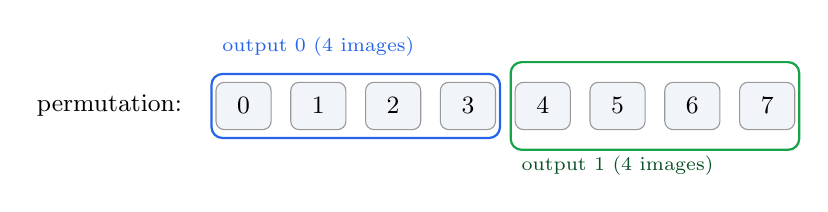
\begin{tikzpicture}[font=\scriptsize,node distance=1.5mm]
  \foreach \i in {0,...,7} {
    \node[blkn,minimum width=7mm,minimum height=6mm] (p\i) at (\i*0.95,0) {\i};
  }
  \node[left=3mm of p0,font=\small] {permutation:};
  % window for output 0 (R=4): 0..3
  \draw[accent,thick,rounded corners] ($(p0.north west)+(-0.05,0.1)$) rectangle ($(p3.south east)+(0.05,-0.1)$);
  \node[accent,above=2mm of p1] {output 0 (4 images)};
  % window for output 1: 4..7
  \draw[green,thick,rounded corners] ($(p4.north west)+(-0.05,0.25)$) rectangle ($(p7.south east)+(0.05,-0.25)$);
  \node[green!50!black,below=2mm of p5] {output 1 (4 images)};
\end{tikzpicture}
\end{center}

\noindent At the default $R=4$ (``stock YOLO''), the width-4 windows \emph{tile} the
permutation: every output uses four distinct images with zero reuse. Lowering $R$ makes
the windows overlap, so each image is reused in $4/R$ outputs with varied partners --- less
decode work, slightly less diversity. Crucially, the number of \emph{training samples} per
epoch is unchanged; $R$ only changes how many source images are decoded.

\begin{pitfall}
The \code{padded\_batch} step pads polygon rows with $-1.0$, \emph{not} the default
$0.0$. Why? $0.0$ is a perfectly valid top-left vertex coordinate --- zero-padded rows
would be read as real vertices and corrupt the polygon target. The value $-1.0$ is the
reserved ``no vertex here'' sentinel throughout the codebase.
\end{pitfall}

\section{Flip and color}
\guidefig{fig_flip_hsv.png}{1.0}{Horizontal flip (real \code{random\_horizontal\_flip} ---
note the box and polygon x-coordinates flip too) and two draws of HSV jitter (real
\code{hsv\_augment}). The brightness term here is \emph{additive}, a deliberate match to the
original codebase. HSV and Albumentations actually run per-batch on the GPU at train time;
this figure calls the same functions directly to show what they do.}

\section{Merging the distance dataset}
Here is the cleverest part of the pipeline. Distance labels come from a \emph{different}
dataset (\code{servingbot\_polygon}) than detection. Rather than build a separate training
job, the two streams are zipped and concatenated on the \textbf{batch dimension}:

\begin{center}
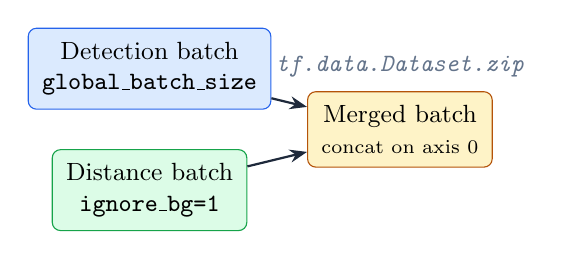
\begin{tikzpicture}[node distance=5mm and 8mm,font=\small]
  \node[blk] (det) {Detection batch\\\scriptsize \code{global\_batch\_size}};
  \node[blkg,below=of det] (dis) {Distance batch\\\scriptsize \code{ignore\_bg=1}};
  \node[blka,right=20mm of $(det)!0.5!(dis)$] (merge) {Merged batch\\\scriptsize concat on axis 0};
  \draw[ar] (det) -- (merge);
  \draw[ar] (dis) -- (merge);
  \node[lbl,above=0.5mm of merge] {\code{tf.data.Dataset.zip}};
\end{tikzpicture}
\end{center}

\noindent The merged batch flows through the same model. Distance-only samples carry
\code{ignore\_bg=1}, which tells the loss to skip class supervision on them (they have no
detection labels). This stream is \textbf{training only} --- there is no distance
validation path, so the distance head is trained but not scored during validation.

\begin{hood}
Three shuffle stages use \emph{distinct} seeds (\code{seed}, \code{seed+1},
\code{seed+2}): the detection source shuffle, the copy-paste source shuffle, and the
post-unbatch shuffle. Distinct seeds keep the stages decorrelated --- a shared seed would
pair the same images every epoch and partially undo each shuffle's job.
\end{hood}

\chapter{Polygons: the PolyYOLO radial representation}
\label{ch:polygons}

The polygon head is the most distinctive part of this codebase, so it gets its own
chapter. The goal: predict an object's outline as 24 points, cheaply enough to be just
three small per-pixel heads.

\section{The radial idea}
Instead of storing 24 arbitrary $(x,y)$ points, PolyYOLO fixes the \emph{angles} and
predicts only the \emph{radii}. Imagine standing at the object's box center and shooting
24 rays outward, one every $15^\circ$ ($360^\circ / 24$). For each ray, predict how far
the boundary is. That distance is the only number you need per vertex --- the angle is
implied by the bin index.

\guidefig{fig_radial.png}{1.0}{The radial encoding. Left: 24 angular bins ($15^\circ$
each) around the box center; the green segment in each occupied bin is the encoded radius
to the polygon boundary (blue). Right: the per-bin target --- a radius (\code{dist}) and a
validity flag (\code{conf}) for each of the 24 bins. This is exactly the target built for
the loss.}

\begin{hood}
Each vertex is actually \emph{three} numbers, so the target is \code{[24 $\times$ 3] = 72}
values per object, interleaved as \code{[dist, angle, conf]}:
\begin{itemize}[leftmargin=1.4em,itemsep=1pt]
  \item \code{dist} --- the radius (how far the boundary is along this ray);
  \item \code{angle} --- a \textbf{sub-bin offset} in $[0,1)$: the exact vertex angle is
        $(i + \text{offset})\cdot15^\circ$, so the vertex isn't snapped to the bin center;
  \item \code{conf} --- 1 if this bin holds a vertex, 0 if empty.
\end{itemize}
This is built in \file{losses/tal\_loss.py}\,:\,\code{\_polygon\_loss}. The three model
heads \code{poly\_dist}, \code{poly\_angle}, \code{poly\_conf} predict these channels.
\end{hood}

\begin{teacher}
Why a sub-bin offset instead of just the bin index? With $15^\circ$ bins, snapping every
vertex to its bin center would quantize the outline coarsely. The offset recovers the
\emph{exact} angle within the bin, so the 24 vertices can sit anywhere on the boundary ---
much smoother outlines for the same 24 bins.
\end{teacher}

\section{Why confidence sees every bin}
Not every object has a vertex in every direction (a thin object leaves many bins empty).
The \code{conf} channel is the gate that decides, at decode time, which bins emit a vertex
(threshold $0.4$).

\begin{why}
The \code{conf} loss is averaged over \textbf{all 24 bins} (occupied $\rightarrow$ 1, empty
$\rightarrow$ 0), while \code{dist} and \code{angle} are averaged over occupied bins only.
The reason is subtle and was found the hard way: \code{conf} is the gate, so it must be
\emph{trained on negatives} (empty bins) to learn to output low confidence there. An
earlier version masked \code{conf} to occupied bins only --- so empty bins never got a
``you should be off'' signal, their confidence drifted above the $0.4$ threshold, and the
decoder emitted spurious vertices: the ``spiky star'' artifacts seen in validation
overlays. \code{dist}/\code{angle} stay masked because a radius/angle on an empty bin is
undefined --- there is no vertex to regress toward.
\end{why}

\section{Arc-length resampling: making bins track real shapes}
There is a catch. Datasets often store polygons with few vertices --- a rectangle might be
just its 4 corners. Drop 4 corners into 24 angular bins and only $\sim$4 bins get a
vertex; the radial target becomes a diamond, and the long edges (which cross many empty
bins) are never learned.

\guidefig{fig_resample.png}{0.92}{The fix, run through the real
\code{resample\_polygons}. A 4-corner rectangle (left) is resampled to 64 points spaced
uniformly \emph{along} the contour (right). The new points lie on the edges, so every
angular bin the boundary crosses now gets a vertex --- the rectangle encodes as a
rectangle, not a diamond.}

\begin{hood}
\code{resample\_polygons} (in \file{data\_pipeline/augmentations.py}) walks the closed
contour and places \code{K=64} points at equal arc-length intervals, interpolating
\emph{on the edges} --- it does not just subsample stored vertices. This runs at decode
time (\code{parser.resample\_points: 64}), so every downstream stage carries a compact
\code{[N, 128]} polygon instead of the raw stored width (which can be thousands of
columns).
\end{hood}

\section{Three formats across the stack}
The same polygon wears three different ``costumes'' as it moves through the code. Keeping
them straight is essential.

\begin{center}
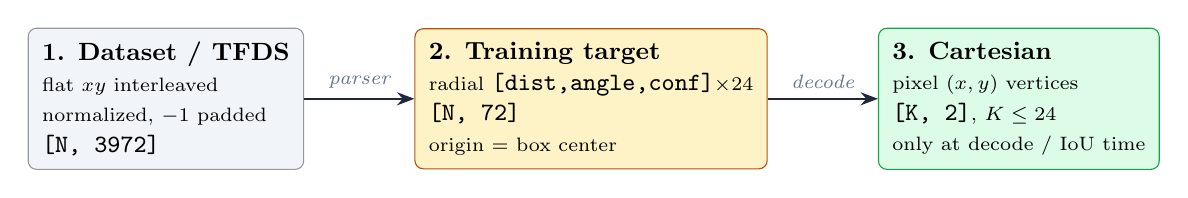
\begin{tikzpicture}[node distance=6mm and 14mm,font=\small]
  \node[blkn,align=left] (a) {\textbf{1. Dataset / TFDS}\\\scriptsize flat $xy$ interleaved\\\scriptsize normalized, $-1$ padded\\\scriptsize \code{[N, 3972]}};
  \node[blka,right=of a,align=left] (b) {\textbf{2. Training target}\\\scriptsize radial \code{[dist,angle,conf]}$\times24$\\\scriptsize \code{[N, 72]}\\\scriptsize origin = box center};
  \node[blkg,right=of b,align=left] (c) {\textbf{3. Cartesian}\\\scriptsize pixel $(x,y)$ vertices\\\scriptsize \code{[K, 2]}, $K\le24$\\\scriptsize only at decode / IoU time};
  \draw[ar] (a)--(b) node[midway,above,lbl]{parser};
  \draw[ar] (b)--(c) node[midway,above,lbl]{decode};
\end{tikzpicture}
\end{center}

\begin{center}
\renewcommand{\arraystretch}{1.25}
\begin{tabular}{l l >{\raggedright\arraybackslash}p{5.4cm}}
\toprule
\textbf{Stage} & \textbf{Shape} & \textbf{Where} \\
\midrule
TFDS input        & \code{[N, 3972]} flat $xy$, $-1$ pad & dataset decoders \\
Training target   & \code{[N, 72]} radial & loss / parser \\
Prediction output & \code{[B, max\_det, 24, 3]} activated & detection generator \\
Cartesian (transient) & \code{[K, 2]} pixels & only at IoU/eval/viz \\
\bottomrule
\end{tabular}
\end{center}

\begin{pitfall}
In the model's \emph{prediction} output, the polygon \code{conf} values are already
sigmoid-activated by the detection generator --- they are \textbf{not} raw logits. Apply
your $0.4$ threshold directly. (And remember validity is keyed off the $-1.0$ sentinel,
not ``$\geq 0$'': a vertex can legitimately be slightly negative after a mosaic overflow
and is still real.)
\end{pitfall}

\section{Decoding a predicted polygon}
At inference, for each bin $i$ whose \code{conf}$_i \geq 0.4$:
\[
\text{angle} = (i + \text{offset}_i)\cdot 15^\circ, \qquad
\text{radius} = \text{dist}_i, \qquad
(x,y) = \text{box center} + \text{radius}\cdot(\cos,\sin)\,\text{angle}.
\]
Bins below threshold are dropped. The result is up to 24 Cartesian vertices, used for
visualization and for the polygon IoU metric.

\begin{teacher}
\textbf{Known limits of the format.} Because the origin is the box center and each bin
keeps only the \emph{farthest} crossing, the radial format cannot represent holes,
interior concavities, or shapes whose center lies outside the polygon. These are
properties of the representation itself, not bugs --- it trades exactness for a compact,
easy-to-predict encoding.
\end{teacher}

\chapter{The model architecture}

Now we open the network itself. It has three parts --- backbone, decoder, heads --- plus a
post-processing stage for inference. Everything is assembled in
\file{models/yolo\_v8.py}\,:\,\code{build\_yolov8}.

\section{Backbone: turning pixels into features}
The backbone is \textbf{CSPDarkNet-V8} (\file{models/backbone.py}), built from \code{C2f}
blocks and an \code{SPPF} block. It is the ``small'' (\code{-S}) size, set by
\code{depth\_scale=0.33} and \code{width\_scale=0.5}. It emits three feature maps, at
levels \code{"3"}, \code{"4"}, \code{"5"} --- strides 8, 16, 32.

\begin{teacher}
A \textbf{C2f block} is YOLOv8's main building block: it splits the channels, runs several
small bottleneck convolutions, and concatenates everything back. This reuses features
cheaply (a ``cross-stage partial'' design). \textbf{SPPF} (Spatial Pyramid Pooling --
Fast) pools the features at several window sizes and stacks them, giving the network a
large receptive field without huge kernels.
\end{teacher}

\begin{pitfall}
Even though the shipped YAML sets \code{depth\_scale: 1.0} and \code{width\_scale: 1.0},
the model is still the \emph{small} one: \code{model\_id: cspdarknetv8s} takes precedence
over those scale fields. Don't be fooled by the \code{1.0}s.
\end{pitfall}

\section{Decoder: the FPN-PAN}
The three backbone maps go into an \textbf{FPN-PAN} decoder (\file{models/decoder.py}),
which fuses information across scales in two passes.

\begin{center}
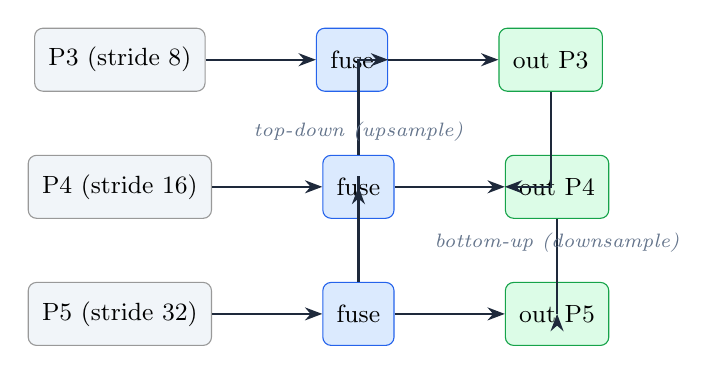
\begin{tikzpicture}[node distance=8mm and 14mm,font=\small]
  % backbone levels
  \node[blkn] (p3) {P3 (stride 8)};
  \node[blkn,below=of p3] (p4) {P4 (stride 16)};
  \node[blkn,below=of p4] (p5) {P5 (stride 32)};
  % top-down
  \node[blk,right=of p5] (t5) {fuse};
  \node[blk,right=of p4] (t4) {fuse};
  \node[blk,right=of p3] (t3) {fuse};
  \draw[ar] (p5)--(t5); \draw[ar] (t5) |- (t4); \draw[ar] (p4)--(t4);
  \draw[ar] (t4) |- (t3); \draw[ar] (p3)--(t3);
  \node[lbl,above=0.5mm of t4] {top-down (upsample)};
  % bottom-up
  \node[blkg,right=of t3] (b3) {out P3};
  \node[blkg,right=of t4] (b4) {out P4};
  \node[blkg,right=of t5] (b5) {out P5};
  \draw[ar] (t3)--(b3); \draw[ar] (b3) |- (b4); \draw[ar] (t4)--(b4);
  \draw[ar] (b4) |- (b5); \draw[ar] (t5)--(b5);
  \node[lbl,below=0.5mm of b4] {bottom-up (downsample)};
\end{tikzpicture}
\end{center}

\noindent The top-down path carries strong semantic signal from coarse levels down to fine
ones; the bottom-up path carries precise localization back up. Each fusion uses a
\code{C2f} stack; activations are ReLU throughout. The output is one fused feature map per
level, fed to the heads.

\section{The six heads}
At every pixel of every level, six small branches predict (\file{models/head.py},
\code{YoloV8Head}):

\begin{center}
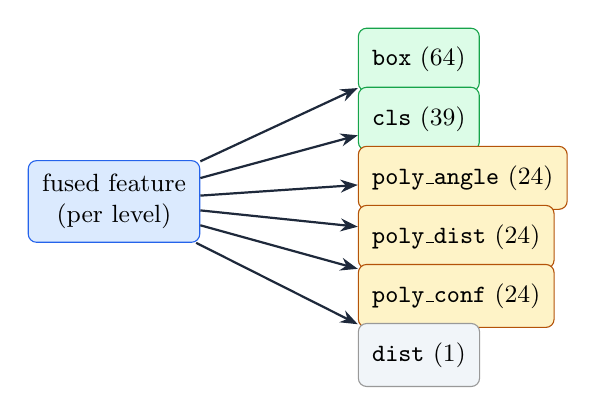
\begin{tikzpicture}[node distance=3mm and 10mm,font=\small]
  \node[blk] (feat) {fused feature\\(per level)};
  \node[blkg,right=20mm of feat,yshift=18mm] (box) {\code{box} (64)};
  \node[blkg,right=20mm of feat,yshift=10.5mm] (cls) {\code{cls} (39)};
  \node[blka,right=20mm of feat,yshift=3mm] (pa) {\code{poly\_angle} (24)};
  \node[blka,right=20mm of feat,yshift=-4.5mm] (pd) {\code{poly\_dist} (24)};
  \node[blka,right=20mm of feat,yshift=-12mm] (pc) {\code{poly\_conf} (24)};
  \node[blkn,right=20mm of feat,yshift=-19.5mm] (di) {\code{dist} (1)};
  \foreach \h in {box,cls,pa,pd,pc,di} \draw[ar] (feat)--(\h);
\end{tikzpicture}
\end{center}

\begin{hood}
\textbf{Smart bias initialization.} The class head's bias is initialized to
$\log\!\big(5 / \text{num\_classes} / (\text{input\_size}/\text{stride})^2\big)$ so that,
before any training, the model predicts a low, sensible object probability per cell (this
stabilizes the first steps). The box bias is set to $1.0$. When warm-starting, only the
backbone and decoder weights load --- the heads start fresh.
\end{hood}

\section{How the box head works: DFL}
The box head does not regress four numbers directly. Each of the four sides
(left, top, right, bottom) is predicted as a \textbf{probability distribution over 16
distance bins}, and the decoded distance is the \emph{expected value} of that distribution.
This is \textbf{Distribution Focal Loss (DFL)}.

\guidefig{fig_dfl.png}{0.72}{DFL: one box side as a softmax over 16 bins. The predicted
distance is $\sum_i p_i \cdot i$ (the expected bin), then multiplied by the level's stride
to get pixels. Predicting a distribution rather than a point lets the model express
uncertainty and yields sharper, better-calibrated box edges.}

\noindent So the \code{box} head's 64 channels are $4 \text{ sides} \times 16 \text{ bins}$.
The decode (softmax $\rightarrow$ expected value) is a fixed $1\times1$ convolution in
\file{models/detection\_generator.py}\,:\,\code{\_decode\_dfl}.

\section{Anchors and strides}
The model is \textbf{anchor-free}: one anchor point per cell, at the cell center
$(i+0.5)\cdot\text{stride}$. The box head predicts the distances from that point to the
four sides; \code{dist2bbox} turns those into corner coordinates. Anchor points are built
on the fly inside the loss and the detection generator --- they are not learned.

\section{Inference: the detection generator}
During training the heads emit raw numbers. For inference (\code{deploy=True}) the
\textbf{detection generator} decodes everything into final results:

\begin{enumerate}[leftmargin=1.4em,itemsep=1pt]
  \item DFL decode $\rightarrow$ \code{xyxy} boxes (times stride);
  \item per-class greedy \textbf{NMS} (\code{max\_boxes=300}, \code{nms=0.65},
        \code{score=0.05});
  \item polygon decode: \code{(conf, dist, angle)} sigmoid/softmax-activated, vertices
        reconstructed for bins above threshold;
  \item distance decode: $\exp$ from log-scale, clipped to $[0.5, 10.0]$ meters.
\end{enumerate}

\begin{teacher}
\textbf{Why log-scale distance?} Predicting $\log(\text{distance})$ instead of raw meters
makes the model's error \emph{relative} --- being off by 0.5\,m matters more for a 1\,m
object than a 9\,m one. The log transform builds that intuition into the loss, and the
output is exponentiated back to meters at decode time.
\end{teacher}

\chapter{The losses}

This chapter is the heart of training. The total loss combines a task-aligned detection
loss with polygon and distance terms. It lives in \file{losses/}, entry point
\file{tal\_loss.py}\,:\,\code{TaskAlignedLossExtended}.

\section{First, the assignment problem}
The model predicts at thousands of grid cells; an image has a handful of objects. Before
we can compute any loss, we must decide \emph{which cells are responsible for which
object}. A bad rule wrecks training. YOLOv8 uses \textbf{Task-Aligned Assignment (TAL)}
(\file{losses/tal\_assigner.py}), which picks the cells whose predictions are already both
well-localized \emph{and} well-classified.

\begin{center}
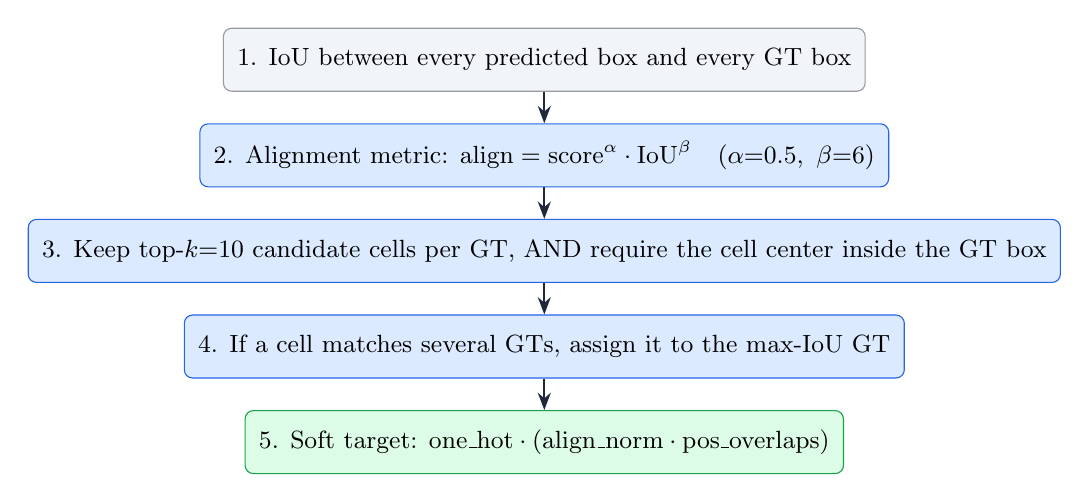
\begin{tikzpicture}[node distance=4mm,font=\small]
  \node[blkn] (iou) {1. IoU between every predicted box and every GT box};
  \node[blk,below=of iou] (al) {2. Alignment metric: $\text{align} = \text{score}^{\alpha}\cdot \text{IoU}^{\beta}$\quad($\alpha{=}0.5,\ \beta{=}6$)};
  \node[blk,below=of al] (tk) {3. Keep top-$k{=}10$ candidate cells per GT, AND require the cell center inside the GT box};
  \node[blk,below=of tk] (dup) {4. If a cell matches several GTs, assign it to the max-IoU GT};
  \node[blkg,below=of dup] (soft) {5. Soft target: $\text{one\_hot}\cdot(\text{align\_norm}\cdot\text{pos\_overlaps})$};
  \foreach \a/\b in {iou/al,al/tk,tk/dup,dup/soft} \draw[ar] (\a)--(\b);
\end{tikzpicture}
\end{center}

\begin{teacher}
``Task-aligned'' means the assignment rewards cells that do \emph{both} jobs well at once.
A cell that draws a tight box but guesses the wrong class --- or names the right class but
in the wrong place --- scores low on $\text{score}^{\alpha}\cdot\text{IoU}^{\beta}$ and is
not chosen. This couples the classification and localization tasks so they improve
together.
\end{teacher}

\begin{hood}
The assignment is computed under \code{stop\_gradient} --- it selects targets but no
gradient flows through the selection. The classification target is \emph{soft}: instead of
a hard 1, the positive class gets \code{align\_norm $\times$ pos\_overlaps}, where
\code{pos\_overlaps} is the per-GT max IoU. This scales the class target by localization
quality, exactly matching the Ultralytics recipe.
\end{hood}

\section{The loss tree}
The total loss is a weighted sum of five families of terms:

\begin{center}
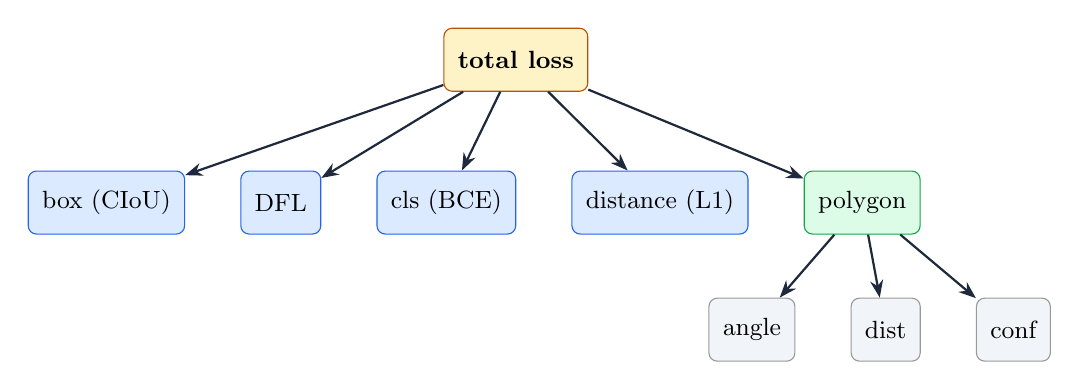
\begin{tikzpicture}[node distance=5mm and 7mm,font=\small]
  \node[blka] (tot) {\textbf{total loss}};
  \node[blk,below=10mm of tot,xshift=-52mm] (box) {box (CIoU)};
  \node[blk,right=of box] (dfl) {DFL};
  \node[blk,right=of dfl] (cls) {cls (BCE)};
  \node[blk,right=of cls] (dist) {distance (L1)};
  \node[blkg,right=of dist] (poly) {polygon};
  \node[blkn,below=8mm of poly,xshift=-14mm] (pa) {angle};
  \node[blkn,right=of pa] (pd) {dist};
  \node[blkn,right=of pd] (pc) {conf};
  \foreach \h in {box,dfl,cls,dist,poly} \draw[ar] (tot)--(\h);
  \foreach \h in {pa,pd,pc} \draw[ar] (poly)--(\h);
\end{tikzpicture}
\end{center}

\subsection{Box: CIoU and DFL}
\textbf{CIoU} is IoU plus penalties for center distance and aspect-ratio mismatch ---
$1-(\text{IoU}-\rho^2/c^2-\alpha v)$ --- a smoother, better-behaved box loss than plain
IoU. \textbf{DFL} trains the 16-bin distributions of the box head toward the true side
distances. Both are weighted per-anchor by how aligned each anchor is, so well-matched
cells dominate the box gradient.

\subsection{Classification}
Binary cross-entropy with logits, summed over the 39 classes. On distance-only samples
(\code{ignore\_bg=1}) the class loss is masked to foreground anchors, since those samples
carry no detection labels.

\subsection{Polygon: three sub-losses}
The polygon terms (\file{losses/polygon\_loss.py}) train the radial target from
Chapter~\ref{ch:polygons}:
\begin{itemize}[leftmargin=1.4em,itemsep=1pt]
  \item \textbf{angle} --- BCE on $\text{sigmoid}(\text{pred})$ toward the sub-bin offset,
        averaged over \emph{valid vertices};
  \item \textbf{dist} --- squared error $(\text{target}-\text{softplus}(\text{pred}))^2$,
        averaged over \emph{valid vertices};
  \item \textbf{conf} --- BCE on per-bin validity, averaged over \emph{all 24 bins}.
\end{itemize}

\subsection{Distance}
L1 error on log-scale distance, masked to entries with a valid distance label
(sentinel $-10.0$ marks ``no distance''), normalized by the total GT object count.

\section{Gains and normalization}
Each term is scaled by a \textbf{gain} from the YAML. But the terms do not share the same
denominator, so the gains are \emph{not} directly comparable across heads --- a crucial
subtlety.

\begin{center}
\renewcommand{\arraystretch}{1.2}
\begin{tabular}{l l l}
\toprule
\textbf{Term} & \textbf{Gain} & \textbf{Normalizer / reduction} \\
\midrule
box CIoU / DFL & 7.5 / 1.5 & \code{target\_scores\_sum}, per-anchor weighted \\
cls            & 0.5 & \code{target\_scores\_sum} \\
distance       & 1.0 & \code{num\_objs} (total batch GT count) \\
poly angle     & 0.4 & \code{num\_objs}, mean over valid vertices \\
poly dist      & 0.45 & \code{num\_objs}, mean over valid vertices \\
poly conf      & 0.2 & \code{num\_objs}, mean over \textbf{all 24 bins} \\
\bottomrule
\end{tabular}
\end{center}

\noindent An overall \code{poly\_gain=0.5} multiplies the summed polygon loss. The
assignment parameters are \code{tal\_alpha=0.5}, \code{tal\_beta=6.0}, \code{topk=10}.

\begin{pitfall}
Because the denominators differ (\code{target\_scores\_sum} for detection vs
\code{num\_objs} for polygon/distance), you cannot reason about relative importance by
comparing gains alone. If you change a masking rule or a reduction, the magnitude of that
term shifts and its gain must be re-tuned. These conventions are pinned by
\file{tests/test\_polygon\_loss\_conventions.py} precisely so they don't drift silently.
\end{pitfall}

\begin{hood}
The loss returns a 9-tuple:
\code{(total, box, dfl, cls, dist, poly, poly\_angle\_raw, poly\_dist\_raw,
poly\_conf\_raw)}. The last three are the un-gained polygon sub-losses, logged separately
to TensorBoard (\code{train/poly\_angle\_loss}, etc.) so you can see \emph{which} polygon
component is misbehaving --- they do not re-enter \code{total}.
\end{hood}

\chapter{Training: optimizer, schedules, and the loop}

We have a model and a loss. This chapter is how the codebase actually \emph{trains} ---
the optimizer, the learning-rate schedule, the weight-averaging trick, and the custom
training loop. The entry point is \file{scripts/run\_train.py}; the loop lives in
\file{train/trainer.py}.

\section{The optimizer: SGD with warmup}
Training uses \textbf{SGD with Nesterov momentum} (\file{optimizers/sgd\_warmup.py}). Two
features make it specific to this codebase.

\guidefig{fig_schedules.png}{1.0}{Left: the learning-rate schedule, computed from the
actual optimizer formulas. The weight group ramps \emph{up} from 0 during warmup, then
follows a cosine decay. The BN/bias groups ramp \emph{down} from $0.1$. Right: the EMA
decay, $\min(0.9999,(1+t)/(10+t))$ --- it starts low (fast averaging) and rises toward
$0.9999$ (slow, stable averaging) as training proceeds.}

\begin{teacher}
\textbf{Warmup} means starting with a tiny learning rate and increasing it over the first
few thousand steps. Fresh weights produce wild gradients; a gentle start avoids blowing up
before the model settles. \textbf{Cosine decay} then smoothly lowers the rate toward the
end so the model fine-tunes into a good minimum.
\end{teacher}

\begin{why}
This optimizer has \textbf{three parameter groups} --- BatchNorm, biases, and weights ---
with different warmup behavior. Unusually, the BN/bias groups \emph{ramp down} from an
absolute LR of $0.1$ (ten times the base) toward the base rate, while weights ramp up from
0. Stock Ultralytics warms biases \emph{up} from a small value. This ramp-\emph{down}
direction matches the original codebase the model was migrated from, and the existing
checkpoints were trained under it --- changing it would mean retraining.
\end{why}

\section{EMA: a smoothed copy of the weights}
The trainer keeps an \textbf{Exponential Moving Average} of the weights
(\file{optimizers/ema.py}). After each step, a shadow copy is nudged toward the current
weights with a decay that grows over time. The EMA weights are usually smoother and
generalize better, so they are \textbf{swapped in for evaluation} and swapped back out
afterward.

\begin{hood}
The decay is dynamic: $\min(0.9999, (1+t)/(10+t))$, incremented before it is read (matching
Ultralytics' \code{ModelEMA}). Evaluation calls \code{swap\_in} before and \code{swap\_out}
after, so reported metrics reflect the averaged weights while training continues on the raw
ones. Warm-starting a new run also loads from the EMA shadows --- they hold the complete
weights, including list-tracked C2f sublayers the plain object graph can miss.
\end{hood}

\section{The training loop and epoch accounting}
The loop is custom (not Orbit) so it can do several project-specific things: swap EMA
weights around validation, merge the detection+distance streams, save checkpoints at epoch
boundaries, handle preemption (SIGTERM), and auto-resume from the newest checkpoint.

\begin{hood}
The training stream is \textbf{infinite}, so an ``epoch'' is defined by the trainer, not by
data exhaustion. It runs exactly \code{steps\_per\_loop} steps per epoch, where
\code{steps\_per\_loop = train\_total\_examples // batch\_size}, from one persistent
iterator. Everything derived is then consistent by construction:
\code{decay\_steps = steps\_per\_loop $\times$ epochs} and
\code{checkpoint\_interval = steps\_per\_loop} (one epoch). After a mid-epoch resume, only
the remainder to the next epoch boundary is run, so boundaries stay at exact multiples.
\end{hood}

\begin{pitfall}
\code{decay\_steps} is an explicit field in the YAML, not derived. If it disagrees with
\code{steps\_per\_loop $\times$ epochs}, the cosine schedule will not finish where the
training does. \code{run\_train.py} \emph{warns} at startup if they diverge --- watch for
that line.
\end{pitfall}

\section{Mixed precision and XLA}
The reference tier runs in \textbf{\code{mixed\_bfloat16}}: most of the network computes in
16-bit \code{bfloat16} (faster, less memory), while the prediction heads and the loss are
pinned to \code{float32} for numerical safety --- so no loss scaling is needed. \textbf{XLA}
(a graph compiler) is an optional A/B toggle. Both are applied in
\code{run\_train.py:\_apply\_runtime\_config} before any op runs.

\begin{teacher}
\textbf{bfloat16} is a 16-bit float with the same exponent range as 32-bit but fewer
mantissa bits. It halves memory and speeds up matmuls on modern GPUs, while its wide range
avoids the overflow problems that plague the older \code{float16}. Keeping the loss in
\code{float32} preserves accuracy where it matters most.
\end{teacher}

\section{Multiple GPUs}
Data-parallel training with \code{MirroredStrategy} is supported and \textbf{numerically
identical} to single-device. The reference config defaults to \code{one\_device} on one
GPU (avoiding MirroredStrategy's overhead). The correctness hinges on two things: the loss
normalizers (\code{num\_objs}, \code{target\_scores\_sum}) are all-reduced to \emph{global}
counts, and gradients are all-reduced across replicas --- both no-ops on a single GPU, so
single-GPU runs are byte-for-byte unchanged.

\section{What you can watch while it trains}
TensorBoard gets rich logging: every scalar carries a markdown description (name +
formula), per-class detection metrics are tagged by class name, the three polygon
sub-losses are logged separately, and \code{train/data\_wait\_ms} vs
\code{train/throughput\_img\_per\_s} let you tell whether the bottleneck is the data
pipeline or the GPU. Augmented training images are logged each epoch under
\code{train/augmentations} (geometry + labels, before the GPU color pass).

\chapter{Configuration: how a run is described}

Everything about a run --- model size, augmentation, gains, schedule --- lives in one
\textbf{experiment YAML}. There is no hidden state; the YAML is the authoritative
hyperparameter source. This chapter explains how it loads and what the main knobs are.

\section{YAML to dataclasses}
\file{configs/yaml\_loader.py}\,:\,\code{load\_config} reads the YAML and maps it onto
plain dataclasses in \file{configs/model\_config.py}. The mapper is \textbf{hand-rolled}
(not \code{dacite}, despite the dependency being listed).

\begin{pitfall}
Unknown keys outside the \code{runtime}/\code{losses} sections are \textbf{silently
ignored}. A typo in a field name will not raise an error --- it just won't take effect. If
a setting seems to do nothing, check the spelling against the dataclass field names.
\end{pitfall}

\subsection{Inheritance}
A config can set \code{base: <path>} to inherit another config and deep-merge its own keys
on top (override wins, dicts merge). For example, the bf16/XLA variant is just a thin
overlay:

\begin{lstlisting}[language=yaml]
base: yolov8_poly_dist.yaml
runtime:
  enable_xla: true
\end{lstlisting}

\section{The structure}
\begin{center}
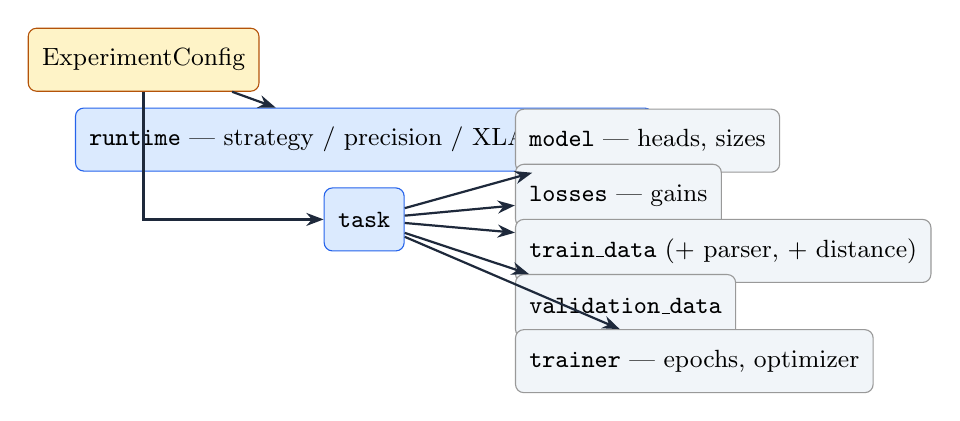
\begin{tikzpicture}[node distance=2mm and 10mm,font=\small]
  \node[blka] (exp) {ExperimentConfig};
  \node[blk,below right=2mm and 6mm of exp.south west,anchor=north west] (rt) {\code{runtime} --- strategy / precision / XLA / threads};
  \node[blk,below=of rt] (task) {\code{task}};
  \node[blkn,right=14mm of task,yshift=10mm] (model) {\code{model} --- heads, sizes};
  \node[blkn,right=14mm of task,yshift=3mm] (loss) {\code{losses} --- gains};
  \node[blkn,right=14mm of task,yshift=-4mm] (tr) {\code{train\_data} (+ parser, + distance)};
  \node[blkn,right=14mm of task,yshift=-11mm] (val) {\code{validation\_data}};
  \node[blkn,right=14mm of task,yshift=-18mm] (trn) {\code{trainer} --- epochs, optimizer};
  \draw[ar] (exp)--(rt); \draw[ar] (exp.south)|-(task);
  \foreach \h in {model,loss,tr,val,trn} \draw[ar] (task)--(\h);
\end{tikzpicture}
\end{center}

\section{The knobs you will touch most}
\begin{center}
\renewcommand{\arraystretch}{1.2}
\begin{tabular}{l l >{\raggedright\arraybackslash}p{6.6cm}}
\toprule
\textbf{Field} & \textbf{Default} & \textbf{What it does} \\
\midrule
\code{model.input\_size} & \code{[672,672,3]} & live model input; smart-bias init assumes it \\
\code{model.num\_classes} & 39 & head width + checkpoint-migration rule \\
\code{model.angle\_step} & 15 & polygon bin size; \code{output\_poly\_size == 360/angle\_step} \\
\code{train\_data.global\_batch\_size} & 128 & detection batch (distance batch merged on top) \\
\code{parser.resample\_points} & 64 & arc-length polygon resample target \\
\code{mosaic.group\_size} & 32 & mosaic source pool per group \\
\code{mosaic.decodes\_per\_output} & 4 & R: 4 = stock YOLO; lower = more reuse, less decode \\
\code{trainer.train\_epochs} & 300 & one epoch = one pass of training samples \\
\code{losses.iou\_gain / cls\_gain / dfl\_gain} & 7.5/0.5/1.5 & detection gains \\
\bottomrule
\end{tabular}
\end{center}

\section{Derived fields --- don't hand-edit}
\code{steps\_per\_loop}, \code{train\_steps}, \code{validation\_steps}, and
\code{checkpoint\_interval} are \emph{computed} from \code{train\_total\_examples} and the
batch sizes. The resolved values print in the startup banner. Editing them by hand only
desynchronizes the schedule.

\section{Validated invariants}
Before training starts, \code{run\_train.py:\_validate\_config} refuses to run if any of
these fail --- a fast, friendly guard against silent misconfiguration:
\begin{itemize}[leftmargin=1.4em,itemsep=1pt]
  \item \code{init\_checkpoint} (if set) exists;
  \item \code{output\_poly\_size == 360 // angle\_step};
  \item \code{group\_size >= 4} and \code{group\_size \% decodes\_per\_output == 0};
  \item \code{output\_dir} is creatable; each referenced TFDS data dir exists.
\end{itemize}
It additionally \emph{warns} (not fatal) if \code{decay\_steps != train\_steps}.

\begin{teacher}
\textbf{Why dataclasses + YAML?} The YAML is what a human edits and version-controls; the
dataclasses give the code type-checked, autocomplete-friendly access with sane defaults.
The loader is the bridge. Keeping all hyperparameters in one declarative file makes runs
reproducible: the config \emph{is} the experiment.
\end{teacher}

\chapter{Evaluation: measuring quality}

How do we know the model is any good? The codebase computes three families of metrics ---
detection, polygon, and distance --- in \file{eval/}. This chapter is a plain-language
glossary, so the numbers in TensorBoard and \code{tools/eval} mean something.

\section{Detection metrics (COCO)}
These follow the standard COCO protocol (\file{eval/coco\_metrics.py}).

\begin{center}
\renewcommand{\arraystretch}{1.25}
\begin{tabular}{l >{\raggedright\arraybackslash}p{9.4cm}}
\toprule
\textbf{Metric} & \textbf{Meaning} \\
\midrule
\code{mAP} & mean Average Precision averaged over IoU thresholds 0.50:0.95 (the headline COCO number) \\
\code{mAP50} & AP at a single, looser IoU threshold of 0.5 \\
\code{AR100} & average recall with up to 100 detections per image \\
\code{F1score50} & macro-averaged peak F1 at IoU 0.5 --- \textbf{the best-checkpoint selection metric} \\
\code{precision50 / recall50} & precision / recall at each class's peak-F1 operating point \\
\bottomrule
\end{tabular}
\end{center}

\begin{teacher}
\textbf{Precision, recall, F1.} Precision = ``of the boxes I predicted, how many were
right?'' Recall = ``of the real objects, how many did I find?'' They trade off as you move
the confidence threshold. \textbf{F1} is their harmonic mean; the ``peak F1'' is the best
balance over the whole curve. \textbf{Average Precision} summarizes the entire
precision--recall curve as one number; \textbf{mAP} averages it over classes and IoU
thresholds.
\end{teacher}

\begin{why}
The best checkpoint is chosen by \code{F1score50}, not \code{mAP}. F1 at a single operating
point reflects deployable detection quality (a threshold you would actually ship), and it
is more stable run-to-run for this multi-task model than the stricter mAP average. The
per-category table (\code{-{}-per\_category}) exposes which few classes drag the macro
average down.
\end{why}

\section{Polygon metrics}
Predictions are matched to ground truth by \textbf{box} IoU $> 0.5$, then the polygon
\textbf{mask} IoU is computed by rasterizing both outlines (\code{cv2.fillPoly}).

\begin{center}
\renewcommand{\arraystretch}{1.25}
\begin{tabular}{l >{\raggedright\arraybackslash}p{9.4cm}}
\toprule
\code{poly\_mIoU} & mean polygon mask IoU over matched pairs --- pure segmentation quality \\
\code{poly\_recall50} & fraction of GT objects matched at box IoU 0.5 \\
\bottomrule
\end{tabular}
\end{center}

\noindent The polygon conf gate ($0.4$) is a single shared constant
(\code{eval/polygon\_metrics.DEFAULT\_POLY\_CONF\_THRESH}) used by both the metric and the
visualization overlays, so they can never disagree.

\section{Distance metrics}
Each GT is matched to its highest-IoU detection ($\geq 0.5$); errors are in meters
(predictions are $\exp$'d from log-space first), split near/far at 5\,m.

\begin{center}
\renewcommand{\arraystretch}{1.2}
\begin{tabular}{l >{\raggedright\arraybackslash}p{8.6cm}}
\toprule
\code{dist\_mae} & mean absolute error, meters \\
\code{dist\_rmse} & root-mean-squared error (penalizes large misses) \\
\code{dist\_absrel} & mean relative error $|\text{pred}-\text{gt}|/\text{gt}$ \\
\code{dist\_*\_near / *\_far} & the same, restricted to $<5$\,m / $\geq5$\,m \\
\bottomrule
\end{tabular}
\end{center}

\begin{pitfall}
Distance is only scored when the eval split carries distance labels. The shipped distance
dataset is \textbf{training-only}, so during normal validation the distance head is
\emph{not} evaluated --- a distance regression would not show up in val metrics. The
evaluator code exists; it simply isn't wired into the default val loop.
\end{pitfall}

\section{Running it}
\begin{lstlisting}[language=bash]
python -m tools.eval \
    --config configs/experiments/yolo/yolov8_poly_dist.yaml \
    --checkpoint /run/ckpt-100000 --split val --per_category
\end{lstlisting}

\noindent Evaluation automatically uses the EMA weights. \code{tools/continuous\_eval.py}
can watch a run directory and evaluate each new checkpoint automatically, appending to
\code{eval\_log.jsonl}.

\chapter{Tools, testing, and on-device export}

A research codebase is more than the model. This chapter surveys the supporting cast:
the runnable scripts, the test suite, checkpoint migration, and the export path that puts
the model on an embedded device.

\section{The scripts you run}
All under \file{tools/} and \file{scripts/}; full details and copy-paste commands are in
\file{docs/scripts.md}.

\begin{center}
\renewcommand{\arraystretch}{1.2}
\begin{tabular}{l >{\raggedright\arraybackslash}p{8.8cm}}
\toprule
\textbf{Command} & \textbf{What it does} \\
\midrule
\code{scripts.run\_train} & launch training (prefer \code{tools/train\_supervisor.sh} for long runs) \\
\code{tools.eval} & COCO / polygon / distance metrics on a checkpoint \\
\code{tools.infer} & draw box + polygon overlays on arbitrary images \\
\code{tools.continuous\_eval} & auto-evaluate new checkpoints in a run directory \\
\code{tools.export\_saved\_model} & host/server SavedModel (NMS baked in, $[0,1]$ input) \\
\code{tools.device.export\_device\_dlc} & on-device SNPE/DLC export \\
\code{tools.checkpoint\_migration} & migrate / warm-start checkpoints \\
\code{tools.benchmark\_pipeline} & data-pipeline throughput \\
\code{tools.pipeline.diagnose\_pipeline} & stage-by-stage pipeline timing \\
\bottomrule
\end{tabular}
\end{center}

\section{Checkpoint migration and warm-starting}
\file{tools/checkpoint\_migration.py} loads weights into the model from an existing
checkpoint, auto-detecting the kind:

\begin{center}
\renewcommand{\arraystretch}{1.2}
\begin{tabular}{l l >{\raggedright\arraybackslash}p{5.0cm}}
\toprule
\textbf{Source} & \textbf{Strategy} & \textbf{What transfers} \\
\midrule
legacy TF2-Vision ckpt & \code{frozen} & backbone + decoder (+ head if classes match) \\
this codebase's own ckpt & \code{native} & requested modules, from EMA weights \\
\bottomrule
\end{tabular}
\end{center}

\begin{pitfall}
Warm-start from a checkpoint that carries EMA (a periodic \code{ckpt-N} or a \code{best\_*}),
\textbf{not} a bare model export. The plain model object graph omits some list-tracked C2f
block variables (a Keras quirk), so only the EMA shadows hold the \emph{complete} weights.
The \code{native} strategy loads via that EMA path for exactly this reason.
\end{pitfall}

\section{Testing}
The \code{pytest} suite (\file{tests/}) runs in \textbf{eager mode} and is split into
\code{unit/} (components --- backbone, decoders, EMA, the assigner, the evaluators),
\code{integration/} (full pipeline, checkpoint migration, a real 2-replica multi-GPU test
on virtual CPU devices), \code{smoke/} (a 10-step training loop), and top-level component
tests (losses, mosaic, parser, polygon preprocessing).

\begin{hood}
Two conventions make the tests trustworthy. (1) Unit/integration tests \textbf{never}
require the real datasets --- they build synthetic tensors inline, so CI runs anywhere.
(2) Tests are \emph{discriminating}: they pin a value or relationship that \emph{fails} on
the buggy behavior and passes once fixed (see \file{tests/test\_loss\_reference\_parity.py}),
rather than merely asserting ``runs without error''.
\end{hood}

\begin{lstlisting}[language=bash]
# fast, no datasets (what CI runs):
pytest tests/unit tests/integration -q
# the multi-GPU test needs a fresh process:
pytest tests/integration/test_multigpu.py -q
\end{lstlisting}

\section{On-device export (Qualcomm SNPE / DLC)}
The model ultimately runs on an embedded device. \file{tools/device/export\_device\_dlc.py}
emits a TensorFlow SavedModel laid out as a \textbf{drop-in replacement} for a legacy
on-device DLC, so the existing SNPE conversion pipeline keeps working unchanged. It differs
from the host export in deliberate ways: it bakes the $/255$ normalization in (the device
feeds raw $[0,255]$ pixels), runs in \code{float32}, emits one raw tensor per head (FPN
levels concatenated), and promotes each head to a cleanly named top-level graph node the
SNPE extractor expects.

\begin{pitfall}
The deployed device decoder stores anchors as $(y,x)$ and expects box channels in
\textbf{y-first} order $[t,l,b,r]$, while the model (and the host code) is x-first
$[l,t,r,b]$. The exporter therefore \textbf{reorders the box channels} by default
(\code{-{}-legacy\_box\_order}). Feeding x-first boxes to the y-first decoder transposes
every box --- the kind of bug that drops on-device accuracy from $0.68$ to $0.19$ while
every shape still looks correct. The exporter's \code{-{}-verify} flag checks this and more.
\end{pitfall}

\chapter{Appendix}

\section{Glossary}
\begin{description}[leftmargin=0pt,style=nextline,itemsep=2pt]
  \item[Anchor-free] each grid cell has one anchor point (its center); the box head
    predicts distances to the four sides, not offsets from preset box shapes.
  \item[Backbone] the convolutional feature extractor (here CSPDarkNet-V8-S).
  \item[bfloat16] a 16-bit float with float32's exponent range; halves memory, no loss
    scaling needed.
  \item[CIoU] complete IoU: IoU plus center-distance and aspect-ratio penalties; the box
    regression loss.
  \item[C2f] YOLOv8's cross-stage-partial block: split channels, run bottlenecks,
    concatenate.
  \item[DFL] Distribution Focal Loss: predict each box side as a softmax over 16 bins;
    decode = expected bin value.
  \item[EMA] exponential moving average of the weights; a smoothed copy used for
    evaluation.
  \item[FPN-PAN] feature-pyramid decoder with a top-down then bottom-up fusion path.
  \item[IoU] intersection over union; overlap measure in $[0,1]$.
  \item[Mosaic] augmentation stitching four images into one $2\times$ canvas, then one warp.
  \item[NMS] non-maximum suppression; removes duplicate overlapping detections.
  \item[PolyYOLO radial format] 24 vertices at fixed $15^\circ$ angles, each storing a
    radius, sub-bin angle offset, and validity flag.
  \item[SkipDecoding] keeps images as encoded JPEG bytes through the shuffle buffer;
    decode happens later in the parallel map.
  \item[SPPF] spatial pyramid pooling (fast); enlarges the receptive field.
  \item[Stride] the down-sampling factor of a feature map (8 / 16 / 32 here).
  \item[TAL] Task-Aligned Assignment: picks responsible cells using
    $\text{score}^{\alpha}\cdot\text{IoU}^{\beta}$.
  \item[yxyx / xyxy] box coordinate orders (y-first vs x-first); this codebase converts
    between them at a known seam.
\end{description}

\section{Where everything lives}
\begin{center}
\renewcommand{\arraystretch}{1.15}
\begin{tabular}{l >{\raggedright\arraybackslash}p{8.8cm}}
\toprule
\textbf{Directory} & \textbf{Contents} \\
\midrule
\file{data\_pipeline/} & decoders, copy-paste, mosaic, augmentations, parsers, the distance merge \\
\file{models/} & backbone, decoder, the 6 heads, detection generator, assembly \\
\file{losses/} & TAL assigner, the total loss, polygon and distance losses \\
\file{optimizers/} & SGD + warmup, EMA \\
\file{eval/} & COCO, polygon, and distance metrics \\
\file{train/} & the task, the custom trainer, viz utilities \\
\file{configs/} & dataclasses, the YAML loader, the composable YAML fragments \\
\file{scripts/} & \code{run\_train.py} entry point \\
\file{tools/} & eval, export, migration, benchmarking, device export, diagnostics \\
\file{tests/} & unit / integration / smoke / component tests \\
\file{docs/} & the developer documentation this guide is built from \\
\bottomrule
\end{tabular}
\end{center}

\section{Design decisions worth remembering}
A handful of choices differ from stock YOLOv8 on purpose (see
\file{docs/design\_register.md} for the full list and reasoning):

\begin{itemize}[leftmargin=1.4em,itemsep=2pt]
  \item Training \emph{filters} crowd annotations, while COCO eval \emph{counts} them ---
    matching the original PolyYOLO protocol.
  \item HSV brightness jitter is \emph{additive}, not multiplicative.
  \item The BN/bias warmup LR ramps \emph{down} from $0.1$.
  \item Polygon \code{conf} loss covers \emph{all 24 bins}; \code{angle}/\code{dist} cover
    occupied bins only.
  \item Polygon vertices are \emph{arc-length resampled} to 64 points at decode time.
  \item Mosaic uses the \emph{canvas} formulation (one warp), measured fastest on the
    target CPU.
  \item $-1.0$ is the reserved polygon sentinel; validity is ``$> -1.0$'', never
    ``$\geq 0$''.
\end{itemize}

\noindent Several of these affect \emph{training}: the data and optimization the existing
checkpoints were trained under depend on them, so changing one means retraining. That is
the thread running through this whole codebase --- it is a working, trained system, and its
non-obvious choices are load-bearing.

\vspace{1cm}
\begin{center}
\textit{This guide was generated from the project's own source and documentation.\\
Edit \file{chapters/*.tex} and rebuild with \file{build.sh} to keep it current.}
\end{center}


\end{document}
